\section{\lr{Data and Methodology}}



\subsection{\lr{Data and Sample}}
\begin{itemize}
	\item 
	داده های قیمت، حجم و دیگر مشخصات حسابداری و بازاری شرکت ها از سایت کدال و tsetmc
	\item
	داده منحصر به فرد مالکیت های بالای یک درصد روزانه شرکت ها بورسی از سایت 
	tsetmc
	\item 
	حذف داده های صندوق های سرمایه گذاری معامله پذیر
	\item 
	از تاریخ 
	1393/01 (2014/03)
	 تا تاریخ 
	 1398/12 (2020/03)
	 

	\item 
	گروه های کسب و کار یکی از مشخصات بازار ایران است
		\item 
	داده های گروه های کسب و کار از مقاله
	\lr{\cite{Aliabadi2022}}
	\begin{itemize}
		\item 
		داده های گروه های کسب و کار در ایران مشخص نیست
		\item
		با استفاده از الگوریتم 
		\lr{\cite{almeida2011structure}}
		با آستانه 40\%
		
	\end{itemize}
	\item
	جدول 
	\ref{t2-1}
	مشخصات آماری داده های مالکیت
\end{itemize}
%داده های مالکیت، قیمت، حجم و دیگر متغیر های بازاری و حساب داری شرکت ها از سایت کدال و شركت مديريت فناوري بورس تهران جمع آوری شده است. علاوه بر این به داده های منحصر به فرد 


\begin{LTR}
\lr{	 \begin{table}[htbp]
        \centering
        \caption{ This table reports summary statistics of ownership features for all the listed firms. At this table by group, we mean business groups.}
        \label{t2-1}
        \resizebox{1\textwidth}{!}
        {
        \begin{tabular}{lrrrrrr}
\toprule
Year &  2014 &  2015 &  2016 &  2017 &  2018 &  2019 \\
\midrule
No. of Firms                        &   365 &   376 &   446 &   552 &   587 &   618 \\
No. of Blockholders                 &  1606 &  1676 &  2099 &  2978 &  3374 &  3416 \\
No. of Groups                       &    38 &    41 &    43 &    44 &    40 &    43 \\
No. of Firms in Groups              &   249 &   268 &   300 &   336 &   346 &   375 \\
Ave. Number of group Members        &     7 &     7 &     7 &     8 &     9 &     9 \\
Ave. ownership of each Blockholders &    18 &    19 &    18 &    17 &    18 &    19 \\
Med. ownership of each Blockholders &     5 &     4 &     4 &     4 &     4 &     4 \\
Ave. Number of Owners               &     7 &     6 &     6 &     7 &     7 &     7 \\
Ave. Block. Ownership               &    77 &    77 &    75 &    76 &    75 &    72 \\
\bottomrule
\end{tabular}

         }
      \end{table}}
\end{LTR}



\subsection{\lr{Pair composition} }
\begin{itemize}
	\item 
	حداقل یک مالک مشترک که 
		\item 
		612 شرکت حداقل یک مالک مشترک با دیگر شرکت ها داشتند
	\item 
	93442 جفت که 25 درصد از جفت های ممکن
	$ (612*611)/2 = 373932$

	\item 
	جدول
	 \ref{t2-2}
	 خلاصه آماری جفت های تشکیل شده
	\item 
	برای قرار گرفتن شرکت ها در گروه های کسب و کار 
	\begin{itemize}
		\item
		 چند حالت امکان دارد 
		 \item
		 در شکل 
		 \ref{g2-1}
		 حالت های مختلف بیان شده است
	\end{itemize}
	
\end{itemize}

 
\begin{LTR}
	\lr{  \begin{table}
  \centering
  \caption{ This table reports summary statistics of ownership features for total pairs. At this table by group, we mean business groups.}
  \label{t2-2}
    \resizebox{1\textwidth}{!}
          {
 \begin{tabular}{lrrrrrr}
\toprule
year &   1393 &   1394 &   1395 &   1396 &   1397 &   1398 \\
\midrule
No. of Pairs                          &  20876 &  21187 &  27784 &  41449 &  47234 &  67232 \\
No. of Groups                         &     37 &     40 &     42 &     43 &     39 &     43 \\
No. of Pairs not in Groups            &  11452 &  11192 &  15351 &  26530 &  29182 &  43433 \\
Number of Pairs not in the same Group &   7962 &   8731 &  10971 &  12916 &  15366 &  20745 \\
Number of Pairs in the same Group     &    923 &    955 &   1099 &   1260 &   1536 &   1774 \\
Average Number of Common owner        &      1 &      1 &      1 &      1 &      1 &      1 \\
Med. Number of Common owner           &      1 &      1 &      1 &      1 &      1 &      1 \\
Average Percent of each blockholder   &     19 &     19 &     19 &     19 &     19 &     20 \\
Med. Percent of each blockholder      &     13 &     12 &     12 &     12 &     12 &     14 \\
Average Number of Pairs in one Group  &     31 &     30 &     30 &     34 &     39 &     44 \\
Med. Number of Pairs in one Group     &      8 &     10 &      8 &     10 &      9 &     10 \\
Average Number of Owners              &      5 &      5 &      5 &      5 &      4 &      5 \\
Med. Number of Owners                 &      5 &      5 &      5 &      5 &      4 &      5 \\
Average Block. Ownership              &     73 &     73 &     72 &     70 &     70 &     70 \\
Med. Block. Ownership                 &     73 &     73 &     73 &     71 &     71 &     71 \\
\bottomrule
\end{tabular}

   }
    \end{table} }
\end{LTR}

\begin{figure}[htbp]
	\centering
	\caption{ \lr{Three categories for pairs base on being in business groups}}
	\label{g2-1}
	
	\normalcolor
	\begin{subfigure}[t]{0.9\linewidth}
		
		\resizebox{0.49\textwidth}{!}{
			\begin{tikzpicture}[node distance=2cm]
				
				
				
				\node (CH) [process,yshift = -2cm ,xshift=3.5cm] {Common Owner};
				
				\node (end) [startstop1,left of = CH ,xshift=-1.5cm ] {$ \text{Firm A} $};
				
				\node (end2) [startstop1,right of = CH ,yshift=0cm,xshift=1.5cm] {$ \text{Firm B} $};
				
				\node (sur) [startstop2 ,below of = end ,yshift=0cm,xshift=0cm] {$ \text{Firm X} $};
				
				\node (sur2) [startstop2,below of = end2 ,yshift=0cm,xshift=0cm] {$ \text{Firm Y} $};
				
				
				\draw [arrow] (end) --(sur);
				\draw [arrow] (end2) -- (sur2);
				
				
				\draw [arrow] (CH) -- (sur);
				\draw [arrow] (CH) -- (sur2);
				
				\draw [latex'-latex'] (sur) to [bend right =0]  node[sloped, anchor=center, below] {} (sur2);
				
				
			\end{tikzpicture}
		}   
		\hfill
		\resizebox{0.49\textwidth}{!}{
			\begin{tikzpicture}[node distance=2cm]
				
				
				\node (start) [startstop] { $ \text{Ultimate Owner} $};
				
				
				\node (CH) [process, below of = start,xshift=3.5cm] {Common Owner};
				
				\node (end) [startstop1,below of = start ] {$ \text{Firm A} $};
				
				\node (end2) [startstop1,right of = CH ,yshift=0cm,xshift=1.5cm] {$ \text{Firm B} $};
				
				\node (sur) [startstop2 ,below of = end ,yshift=0cm,xshift=0cm] {$ \text{Firm X} $};
				
				\node (sur2) [startstop2,below of = end2 ,yshift=0cm,xshift=0cm] {$ \text{Firm Y} $};
				
				
				
				\draw [arrow] (start) --(end);
				
				\draw [arrow] (end) --(sur);
				\draw [arrow] (end2) -- (sur2);
				
				\draw [dash dot,->] (start) -- (CH);
				
				\draw [arrow] (CH) -- (sur);
				\draw [arrow] (CH) -- (sur2);
				
				\draw [latex'-latex'] (sur) to [bend right =0]  node[sloped, anchor=center, below] {} (sur2);
				
				
			\end{tikzpicture}
		}
		\caption{ \lr{Pair not in the business group}}
	\end{subfigure}
	\bigskip
	\begin{subfigure}[t]{.45\linewidth}
		\centering
		\tiny
		\resizebox{1\textwidth}{!}{
			
			\begin{tikzpicture}[node distance=2cm]
				
				
				\node (start) [startstop] { $ \text{Ultimate Owner A} $};
				\node (start2) [startstop,right of = start,xshift=5cm] {$ \text{Ultimate Owner B} $};
				
				
				\node (CH) [process, below of = start2,xshift=-3.5cm] {Common Owner};
				
				\node (end) [startstop1,below of = start ] {$ \text{Firm A} $};
				
				\node (end2) [startstop1,below of = start2 ,yshift=0cm,xshift=0cm] {$ \text{Firm B} $};
				
				\node (sur) [startstop2 ,below of = end ,yshift=0cm,xshift=0cm] {$ \text{Firm X} $};
				
				\node (sur2) [startstop2,below of = end2 ,yshift=0cm,xshift=0cm] {$ \text{Firm Y} $};
				
				
				
				\draw [arrow] (start) --(end);
				\draw [arrow] (start2) -- (end2);
				
				\draw [arrow] (end) --(sur);
				\draw [arrow] (end2) -- (sur2);
				
				\draw [dash dot,->] (start) -- (CH);
				\draw [dash dot,->] (start2) -- (CH);
				
				\draw [arrow] (CH) -- (sur);
				\draw [arrow] (CH) -- (sur2);
				
				\draw [latex'-latex'] (sur) to [bend right =0]  node[sloped, anchor=center, below] {} (sur2);
				
				
			\end{tikzpicture}
		}   
		\caption{\lr{ Pair in two distinct business group}}
	\end{subfigure}
	\begin{subfigure}[t]{.45\linewidth}
		\centering
		\tiny
		\resizebox{1\textwidth}{!}{
			
			\begin{tikzpicture}[node distance=2cm]
				
				
				\node (start) [startstop] {Ultimate Owner};
				
				
				
				\node (end) [startstop1,below of = start , yshift=0cm , xshift=-3.5cm ] {$ \text{Firm A} $};
				\node (end2) [startstop1,below of = start , yshift=0cm , xshift=3.5cm ] {$ \text{Firm B} $};
				
				
				
				\node (sur) [startstop2 ,below of = end ,yshift=0cm,xshift=0cm] {$ \text{Firm X} $};
				
				
				\node (sur2) [startstop2 ,below of = end2 ,yshift=0cm,xshift=0cm] {$ \text{Firm Y} $};
				
				
				\node (CH) [process, below of = start ,xshift=0] {Common Owner};
				
				
				\draw [arrow] (start) --(end);
				\draw [arrow] (end) --(sur);
				
				\draw [arrow] (start) --(end2);
				
				\draw [arrow] (end) --(sur);
				\draw [arrow] (end2) -- (sur2);
				
				
				\draw [arrow] (CH) -- (sur);
				\draw [arrow] (CH) -- (sur2);
				\draw [dashed ,->] (start) --(CH);
				
				\draw [latex'-latex'] (sur) to [bend right =0]  node[sloped, anchor=center, below] {} (sur2);
				
				
			\end{tikzpicture}
		} 
		
		\caption{ \lr{Pair in the same business group}}
	\end{subfigure}
	
	
	
\end{figure}  

%
% Figure \ref{g2-2} shows the time series of unique pairs' number in each month. The pattern shows that the portion of pairs that are in one business group is roughly stable. The number of pairs in each period is between 322 to 5101 pairs which, on average, there are 4325 pairs.
% 
% \normalcolor
 
%\begin{figure}[htbp]
%\caption{ The number of unique pairs in each month}
%\label{g2-2}
%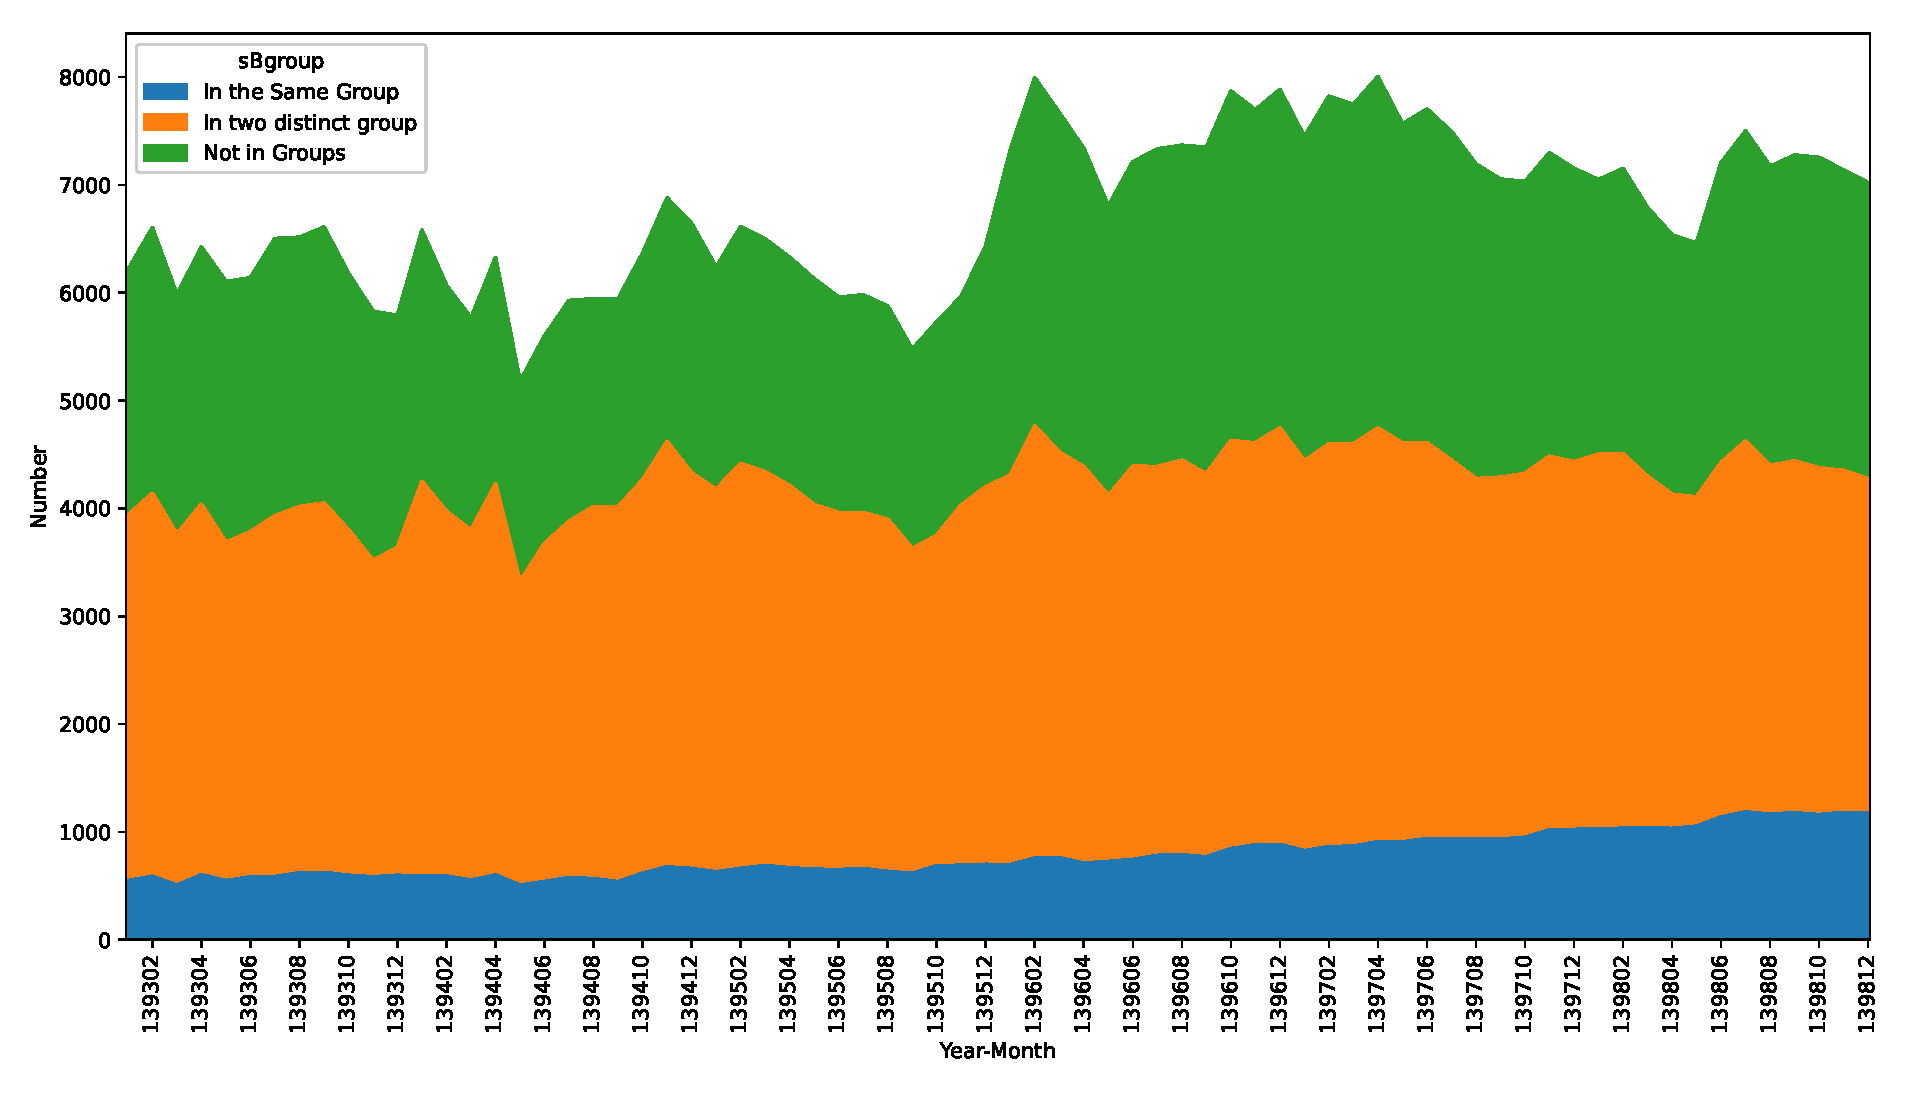
\includegraphics[width=\linewidth]{Output/idMonth.eps}
%\end{figure}
 
  \FloatBarrier
  
  
\subsection{\lr{Measurement of common-ownership}}

\begin{itemize}
	\item 
	جدول 
	\ref{maasurmentsSummary}
	خلاصه ملاک های استفاده شده در ادبیات
	\item 
	دو دسته ملاک اندازه گیری مالکیت مشترک
	\begin{itemize}
		\item 
		دارای پشتوانه مدل
		\begin{itemize}
			\item 
			توضیح تئوری دارند
			\item 
			تفسیر اقتصادی بهتری دارند
			\item 
			جهت دار
			\item
			در سطح صنعت یا شرکت
			\item
		\lr{	(e.g, \cite{harford2011institutional}; \cite{azar2018anticompetitive}; \cite{gilje2020s})}
		\end{itemize}
		\item 
	مدل های بدون پشتوانه
	\begin{itemize}
		\item 
		تفسیر اقتصادی مشخصی ندارند
		\item 
		شک است که چگونه انگیزخ مدیران را اندازه می گیرند
		\item 
		ویژگی های نامطلوبی دارند 
		\item
		محاسبه ساده است
		\item
		در سطح جفت و بدون جهت می توان محاسبه شود
		
		\item
		\lr{(e.g, \cite{AntonPolk}; \cite{azar2011new}; \cite{freeman2019effects}; \cite{hansen1996externalities};  \cite{he2017product}; \cite{he2019internalizing}; \cite{lewellen2021does}; \cite{newham2018common})}
	\end{itemize}
	
		
	\end{itemize}
	
	\item 
	هدف اصلی بررسی اثر مالکیت مشترک بر هم حرکتی در سطح جفت است
	
	\item 
	برای این هدف نیاز به ملاک در سطح جفت بدون جهت است با تفسیر اقتصادی مناسب
	
	\item 
	ملاک
	\cite{AntonPolk}
	میزان درصد مالکیت مشترک از مارکت دو شرکت است
	
	
	\item 
	از این ملاک استفاده می کنیم ولی مشکلی دارد
	\item 
	این ملاک توزیع مالکیت را در نظر نمی گیرد
		\item 
		برای همین از این ملاک استفاده می کنیم
		\begin{equation}
			\text{Overlap}_{Sqrt}(i, j) =  [\frac{\sum_{f =1}^{F}(\sqrt{S^f_{i,t}P_{i,t}}+\sqrt{S^f_{j,t}P_{j,t}})}{\sqrt{S_{i,t}P{i,t}} + \sqrt{S_{j,t}P{j,t}}}]^2 
			\label{sqrt0}
		\end{equation}
		\item
		در بخش 
		\ref{ModifiedMeasure}
		دلیل انتخاب این ملاک بیان شده است
\end{itemize}

\begin{LTR}
	\lr{\begin{table}[htbp]
	\centering
	\scriptsize
	\caption{ This table summarizes common ownership measurements in the literature.}
	\label{maasurmentsSummary}
	\resizebox{\textwidth}{!}{
		\begin{tabular}{cllc}
	\hline\hline
	\multicolumn{1}{c}{Group}      & \multicolumn{1}{c}{Paper} & \multicolumn{1}{c}{measurment} & \multicolumn{1}{c}{Flaws} \\
	\hline\hline
	\addlinespace
	\multicolumn{1}{c}{\multirow{5}[2]{*}{Model Based}} &  \cite{harford2011institutional}     &  \scriptsize  $
	\sum_{i\in I^{A,B}}\frac{\alpha_{i,B}}{\alpha_{i,A} + \alpha_{i,B}}     $     & Bi-directional \\
	\addlinespace 
	&  \cite{azar2018anticompetitive}     &  $   \sum_{j} \sum_k s_j s_k \frac{\sum_i \mu_{ij} \nu_{ik}}{\sum_i \mu_{ij} \nu_{ij}}   $     & Industry level \\
	\addlinespace
	&  \cite{gilje2020s}     &    $ \sum_{i = 1}^{I} \alpha_{i,A}g(\beta_{i,A})\alpha_{i,B}    $   & Bi-directional  \\
	\midrule
	\addlinespace 
	\multicolumn{1}{c}{\multirow{7}[5]{*}{Ad hoc}} & \cite{he2017product};      &  \multirow{2}{*}{$ \sum_{i\in I^{A,B}} 1 $}     & invariant to the level   \\
	& \cite{he2019internalizing} & & of ‌common ownership \\
	\addlinespace
	&  \cite{newham2018common}     &   $ \sum_{i\in I^{A,B}} min\{\alpha_{i,A},\alpha_{i,B}\} $    & ? \\
	\addlinespace
	& \multirow{2}{*}{   \cite{AntonPolk} }  &  \multirow{2}{*}{ $ \sum_{i\in I^{A,B}} \alpha_{i,A}\frac{\bar{\nu}_A}{\bar{\nu}_A +\bar{\nu}_B } + \alpha_{i,B}\frac{\bar{\nu}_B}{\bar{\nu}_A +\bar{\nu}_B }  $ }   &  Invariant to the  \\
	& & & decomposition of ownership \\
	\addlinespace
	& \cite{freeman2019effects}; & \multirow{2}{*}{ $ \sum_{i\in I^{A,B}} \alpha_{i,A} \times \sum_{i\in I^{A,B}} \alpha_{i,B} $ }&?\\
	&  \cite{hansen1996externalities} & & ?\\
	\hline\hline
\end{tabular}
	}
\end{table}
}

\end{LTR}




\begin{itemize}
	\item 
	در هر روز مالکیت مشترک با ملاک اصلاح شده تولید شده است
	\item 
مقدار میانگین ماهانه آن به عنوان مقدار ماهانه استفاده شده است
	\item 
جدول 
\ref{measureResults}
نتایج محاسبات برای مالکیت مشترک ملاک ساده 
(FCAP)
و اصلاح شده
(MFCAP)

\item
مالکیت مشترک برای گروه های کسب و کار حدودا 5 برابر و برای صنعت یکسان حدودا 3 برابر است

\begin{table}[htbp]
%	\centering
	\caption{ text}
	\label{measureResults}
	\resizebox{\textwidth}{!}
	{
		\begin{LTR}
			\lr{\begin{tabular}{lrrrrrrrrrr}
\toprule
\multirow{2}{*}{Subset}& \multicolumn{5}{c}{MFCAP} & \multicolumn{5}{c}{FCAP} \\
\cmidrule(lr){2-6} \cmidrule(lr){7-11}
&       mean &    std &    min & median &    max &         mean &    std &    min & median &    max \\
\midrule
All               &  0.15 &  0.24 &  0.00 &   0.06 &  4.62 &  0.12 &  0.16 &  0.0 &   0.05 &  0.97 \\
Same Group        &  0.47 &  0.41 &  0.00 &   0.41 &  4.04 &  0.38 &  0.25 &  0.0 &   0.37 &  0.97 \\
Not Same Group    &  0.10 &  0.16 &  0.00 &   0.04 &  2.90 &  0.08 &  0.11 &  0.0 &   0.04 &  0.97 \\
Same Industry     &  0.34 &  0.41 &  0.01 &   0.18 &  4.04 &  0.25 &  0.24 &  0.0 &   0.16 &  0.96 \\
Not Same Industry &  0.12 &  0.19 &  0.00 &   0.05 &  4.62 &  0.10 &  0.14 &  0.0 &   0.05 &  0.97 \\
\bottomrule
\end{tabular}
}
			\end{LTR}
	}
\end{table}


\end{itemize}

  \FloatBarrier
\subsection{\lr{Stock Return comovement}}
\label{comovement}
\begin{itemize}
	\item
	هم حرکتی ماهانه شرکت ها را محاسبه کرده ایم
	\item
	برای محاسبه هم حرکتی از باقی مانده مدل های فاکتوری استفاده کرده ایم
	\item
	با توجه به ویژگی بازار ایران شاخص صنعت را هم به مدل های چند فاکتوری اضافه کرده ایم

\begin{itemize}
	\item 
		\begin{equation}
		\begin{split}
			R_{i,t} =\alpha _{i}&+\beta _{mkt,i}{\mathit {R}}_{M,t} + \beta_{Ind,i}{\mathit {R}}_{Ind,t}+\beta _{HML,i}{\mathit {HML}}_{t} \\
			&+\beta _{SMB,i}{\mathit {SMB}}_{t}+\beta _{UMD,i}{\mathit {UMD}}_{t}+ \varepsilon_{i,t}
		\end{split}
		\label{e5Factor}
	\end{equation}
	\item
	از فاکتور های  [
	\lr{\cite{Carhart4Factor}}
	]
\end{itemize}
	
	\item
	برای محاسبه باقی مانده مدل ها، مدل را برای سه ماه ( از دو ماه قبل) پیش بینی می کنیم و بعد از آن باقی مانده ها را محاسبه می کنیم
	\item
	برای ماه مورد نظر هم بستگی باقی مانده ها را محاسبه می کنیم
	\item
	نتایج برای مدل های مختلف  در جدول
	\ref{tCorr}
	نشان داده شده است
	\item
	از مدل چهار عاملی به علاوه صنعت استفاده کرده ایم
	\begin{itemize}
		\item 
		با توجه به دامنه نوسان از تاخیر های فاکتور ها هم استفاده کردیم ولی نتایج  هم بستگی محاسبه شده تفاوت چندانی با مدل های قبلی نداشت
	\end{itemize}
	
\end{itemize}

     
\begin{LTR}
	\lr{ \begin{table}[htbp]
        \centering
        \caption{\footnotesize This table reports distribution of calculated correlation base on different models.}
        \label{tCorr}
        \resizebox{0.85\textwidth}{!}
        {
        \begin{tabular}{lrrrrr}
\toprule
{} &   mean &    std &  min &  median &  max \\
\midrule
 CAPM + Industry    &  0.018 &  0.205 & -1.0 &   0.018 &  1.0 \\
4 Factor            &  0.031 &  0.206 & -1.0 &   0.027 &  1.0 \\
4 Factor + Industry &  0.014 &  0.204 & -1.0 &   0.012 &  1.0 \\
\bottomrule
\end{tabular}

         }
      \end{table}}
\end{LTR}
      

\FloatBarrier


\subsection{Controls}

\begin{itemize}
	\item 
	هم حرکتی ممکن است ویژگی های شرکت ها ناشی شده باشد
	
	\item 
	اولین دسته کنترل ها برای جفت هاست
	\begin{itemize}
\item 
\textbf{SameIndustry} :
صنعت دو شرکت یکسان باشد
\item 
\textbf{SameGroup}:
دو شرکت در یک گروه کسب و کار قرار بگیرند
\item 
\textbf{CrossOwnership}:
حداکثر درصد مالکیت ضربدری میان دو شرکت
		
	\end{itemize}
	\item 
	جدول
	\ref{SameGroupIndustry}
	نشان داده است $5.7 \%$ از جفت های در یک صنعت
	$6.5 \%$ در یک گروه کسب و کار
	1\% نیز هم در یک گروه و هم در یک صنعت قرار دارد
	\item 
دسته دوم کنترل ها مشخصات شرکت ها را کنترل می کند
\begin{itemize}
	\item \textbf{Size1}:
	نرمالایزد رنک ترنسفرد اندازه شرکت بزرگتر
	
	
	\item \textbf{Size2}:
	نرمالایزد رنک ترنسفرد اندازه شرکت کوچکتر
	
	\item \textbf{BookToMarket1}:
	نرمالایزد رنک ترنسفرد نسبت بوک تو مارکت شرکت بزرگتر
	
	\item \textbf{BookToMarket2}:
		نرمالایزد رنک ترنسفرد نسبت بوک تو مارکت شرکت کوچکتر
	\item \textbf{SameSize}:
	منفی مقدار اختلاف اندازه رتبه صدکی دو شرکت نسبت به اندازه
	\item  \textbf{SameBookToMarket}:
	منفی مقدار اختلاف اندازه رتبه صدکی دو شرکت نسبت به بوک تو مارکت
\end{itemize}
	\item 
	متغیر ها مانند مقاله
	\lr{\cite{AntonPolk}}
	تعریف شده است
	\item
کنترل ها به صورت روزانه محاسبه شده اند و پس از آن میانگین ماهانه استفاده شده است
\item 
جدول 
\ref{ControlsSummary}
خلاصه آماری کنترل ها
\end{itemize}



\begin{LTR}
	\lr{\begin{table}[htbp]
\caption{\scriptsize This table reports the number of pairs in the same industry and business group.}
\label{SameGroupIndustry}
               \centering \scriptsize
         {

    \begin{tabular}{lcc}\hline\hline
    {Type of Pairs} & {Yes} &{No} \\
    \hline
    \addlinespace
    {SameIndustry} & 1760  & 16739 \\
          & \tiny(10\%) & \tiny (90\%) \\
          \addlinespace
{SameGroup} & 1118  & 17381 \\
          & \tiny(6\%) & \tiny (94\%) \\
          \addlinespace
{SameGroup \& SameIndustry} & 492  & 18007 \\
          & \tiny(3\%) & \tiny (97\%) \\    
                
          \hline\hline
    \end{tabular}%
                 }
             \end{table}}
\end{LTR}

\begin{LTR}
	\lr{ \begin{table}[htbp]
 \caption{\scriptsize This table shows the summary statistics of specified controls in empirical studies.}
 \label{ControlsSummary}
               \centering 
               \scriptsize
                \resizebox{\textwidth}{!}  {
    \begin{tabular}{lrrrrrrr}\hline\hline
          & \multicolumn{1}{l}{mean} & \multicolumn{1}{l}{std} & \multicolumn{1}{l}{min} & 25\%  & 50\%  & 75\%  & \multicolumn{1}{l}{max} \\
          \hline
          
          SameIndustry & 0.10  & 0.29  & 0.00  & 0.00  & 0.00  & 0.00  & 1.00 \\
          SameGroup & 0.06  & 0.23  & 0.00  & 0.00  & 0.00  & 0.00  & 1.00 \\
          Size1 & 0.72  & 0.21  & 0.01  & 0.58  & 0.78  & 0.91  & 1.00 \\
          Size2 & 0.43  & 0.25  & 0.00  & 0.23  & 0.42  & 0.62  & 0.99 \\
          SameSize & -0.29 & 0.21  & -0.97 & -0.42 & -0.24 & -0.12 & 0.00 \\
          BookToMarket1 & 0.53  & 0.26  & 0.00  & 0.34  & 0.54  & 0.73  & 1.00 \\
          BookToMarket2 & 0.52  & 0.24  & 0.00  & 0.34  & 0.52  & 0.71  & 1.00 \\
          SameBookToMarket & -0.30 & 0.19  & -0.99 & -0.42 & -0.26 & -0.15 & 0.00 \\
          MonthlyCrossOwnership & 0.01  & 0.05  & 0.00  & 0.00  & 0.00  & 0.00  & 0.96 \\
          
    
    \hline\hline
            \end{tabular}
                 }
             \end{table}}
\end{LTR}
         
         
 


\FloatBarrier

